
\section*{HS/38. feladat: Hőcserélő rendszer}
Pincében falon kívül felszerelt 1/2"-os melegvíz vezetéket samottal szigetelnek. Rajzolja meg, hogyan változik a hőveszteség a szig. vastagságával. $D_{kirt}=$ ?Hogyan alakul a helyzet üvegszálas szig. esetén?

\vspace{5mm}
\noindent
Adatok: 
 
$d_k=0,0215$ m; $t_{fl}=65$ °C

$\alpha=11,6$ W/m$^2$K

$t_{lev}=5$ °C (pincetér hőm.-e)

$\lambda=0,47$ W/mK

$l_\textmd{\textit{ü}}=0,07$"
\begin{figure}[H]
	\begin{center}
		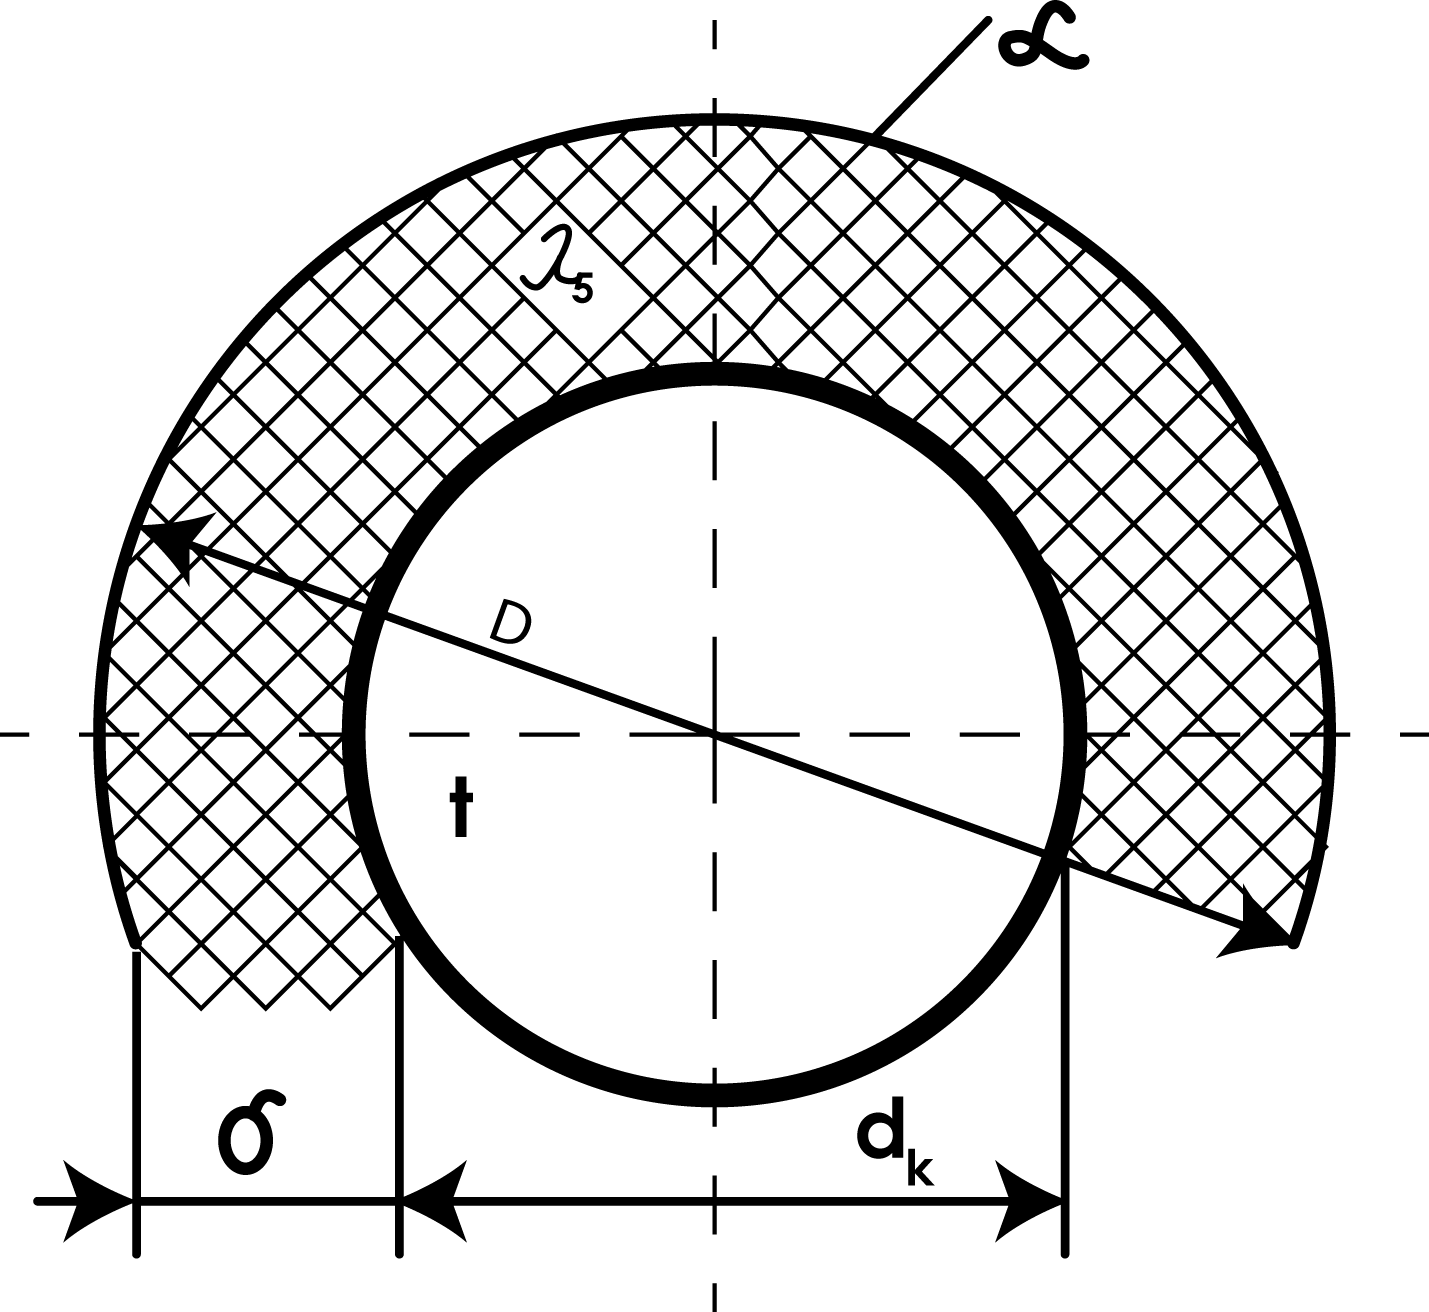
\includegraphics[width=0.5\linewidth]{u9awby123/fig01.png}
	\end{center}
\end{figure}


\vspace{5mm}
\noindent
\textit{Megoldás:}

Gyakorlatban a csőfal termikus ellenállása a szig. mellett elhanyagolható, ennek figyelembevételével a lin. hőáram:

\vspace{5mm}
$q_t=$ \rule{2cm}{0.4pt}

\vspace{5mm}
A kritikus átmérő samottnál: $D_{kritS}=$

üvegsz: $D_{kritÜ}=$

\vspace{5mm}
Meghatározandó egy 1000 kg/h teljesítményű benzollepárló berendezés kondenzátorának hőátadó felülete. A benzol kondenzáziós hőfoka 60 °C, a rendelkezésre álló hűtővíz hőfoka 20 °C, mennyiség 11,0 m$^3$/h. Hőveszteséggel ne számoljunk.

\vspace{5mm}
\noindent
Adatok: 

$G_B=1000$ kg/h . . . benzol tömegárama

$t_B=60$ °C . . . kondenzáció hőfoka

$t_{vk}=20$ °C . . . hűtővíz kezdeti hőfoka

$\dot{V}_v$=11 m$^3$/h . . . hűtővíz kezdeti térfogata

$r_B=3942,2$ kJ/kg . . . benzol rejtett hője (60 °C)


\vspace{5mm}
\noindent
Kérdés: 

a hűtővíz kilépési hőmérséklete . . . $t_{vv}$( °C)

a hőátadási tényező vízoldalon . . . $\alpha_v$ 

a hőátadási tényező benzol oldatban . . . $\alpha_B$

hőátadó felület. . . A(m$^2$)

\vspace{5mm}
\noindent
\textit{Megoldás:}

A víz kilépési hőmérsékletének számítása	

\vspace{5mm}
$\dot{Q}_{\textmd{\textit{á}}tsz}=\dot{G_B}\cdot r_B=\dot{G_v}\cdot c_v (t_{vv}-t_{vk})$

\vspace{5mm}
$t_{vv}=\dfrac{\dot{Q}_B\cdot r_B}{\dot{G}_v\cdot c_v}+t_{vk}=\dfrac{1000\cdot94,2}{11,10^3\cdot1}+20=$\underline{28,50 °C}

\vspace{5mm}
$\Delta t_{\textmd{\textit{köz log}}}=\dfrac{\Delta t_k-\Delta t_v}{\textmd{ln}\frac{\Delta t_k}{\Delta t_v}}=\dfrac{40-31,44}{\textmd{ln}\frac{40}{31,44}}=\dfrac{8,56}{0,2408}=$\underline{35,55 °C}


\begin{figure}[H]
	\begin{center}
		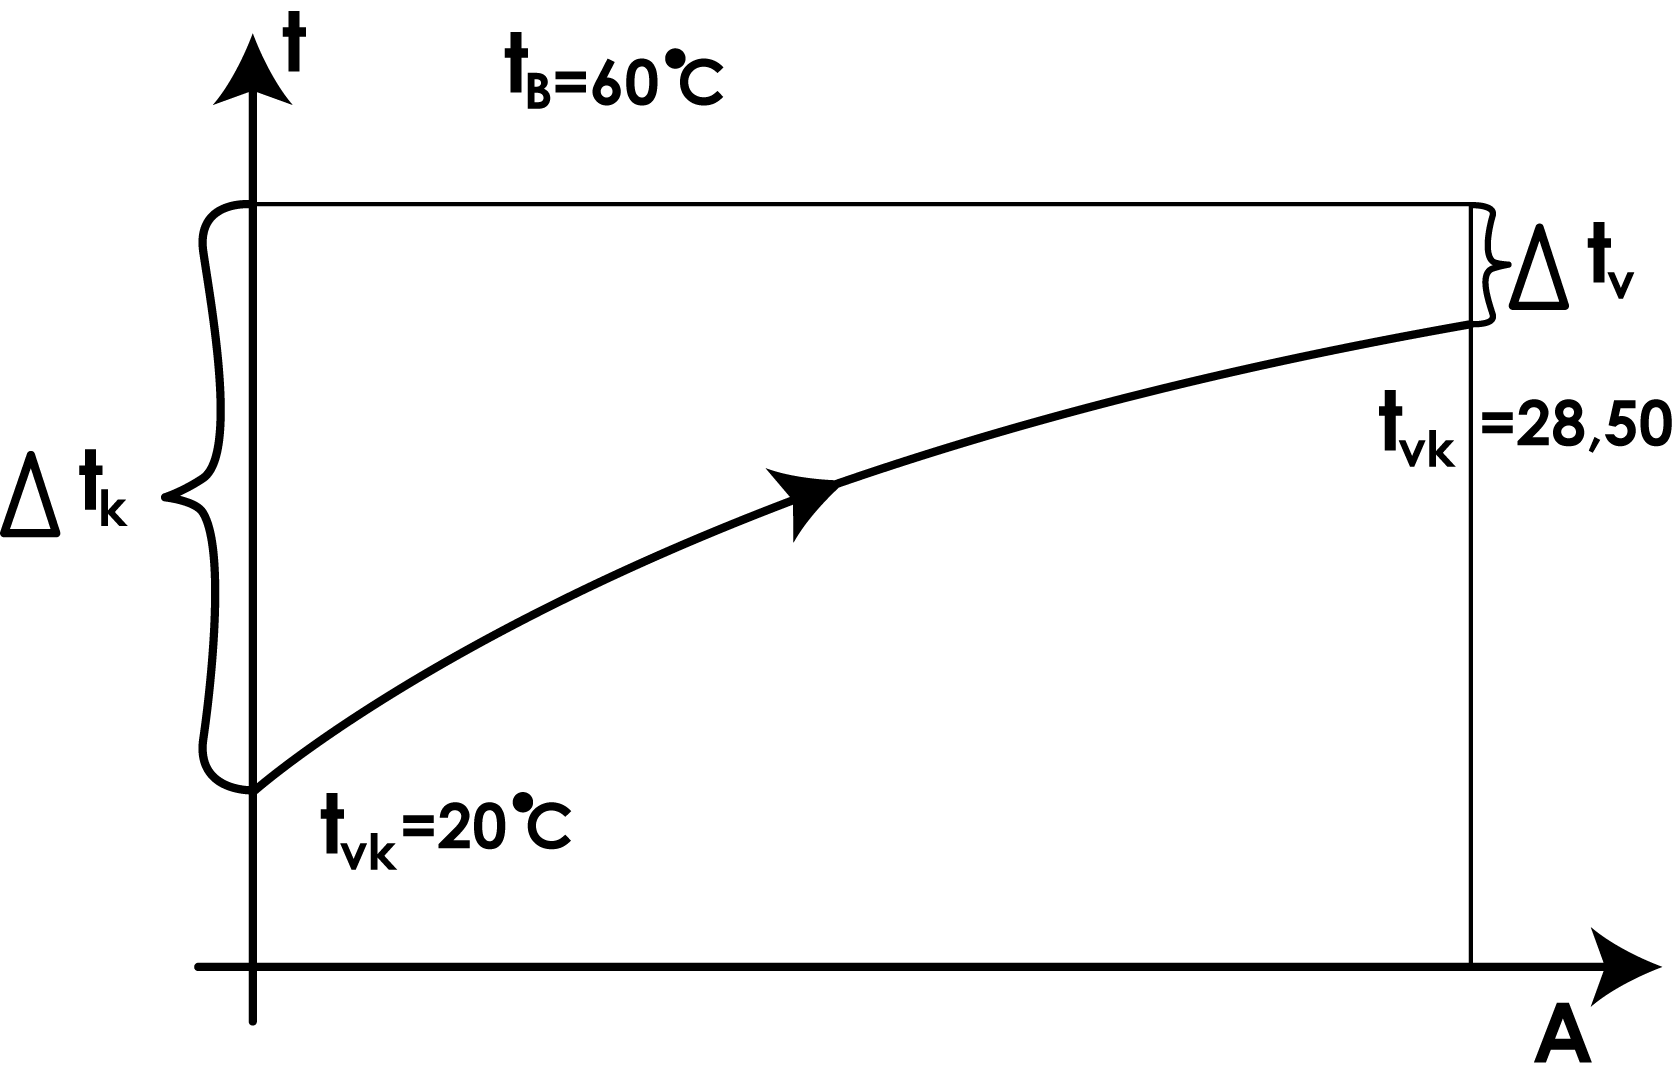
\includegraphics[width=0.5\linewidth]{u9awby123/fig02.png}
	\end{center}
\end{figure}

\vspace{5mm}
\noindent
3. Előzetes becslés alapján legyen a hőátsz. tényezők értéke $\chi'=1160$ W/m$^2$K. Ezzel szükséges átszármaztató felület

\vspace{5mm}
$A$'=$\dfrac{\dot{Q}_{\textmd{\textit{átsz}}}}{\kappa\cdot\Delta t_{\textmd{\textit{köz lg}}}}=\dfrac{394,2\cdot103\cdot1000}{1160\cdot36,55\cdot3600}=2,649m^2=$\underline{2,7m$^2$}

\vspace{5mm}
\noindent
4. Felvesszük a kondenzátor elrendezés. Legyen fekvő elrendezésű, csövek mérete $\qquad \mathbf{\O}$ 25/20, anyaga: sárgaréz 1-2 átfutású

\vspace{5mm}
\noindent

Összes szükséges csőhossz: 

\vspace{5mm}
$l'=\dfrac{A'}{d_{\textmd{belső}}\cdot\pi}=\dfrac{2,7}{0,02\pi}=42,97$ m

\vspace{5mm}
a vázlat szerint csőosztásnál $i=$30db, így hőcserélő hossza

\begin{figure}[H]
	\begin{center}
		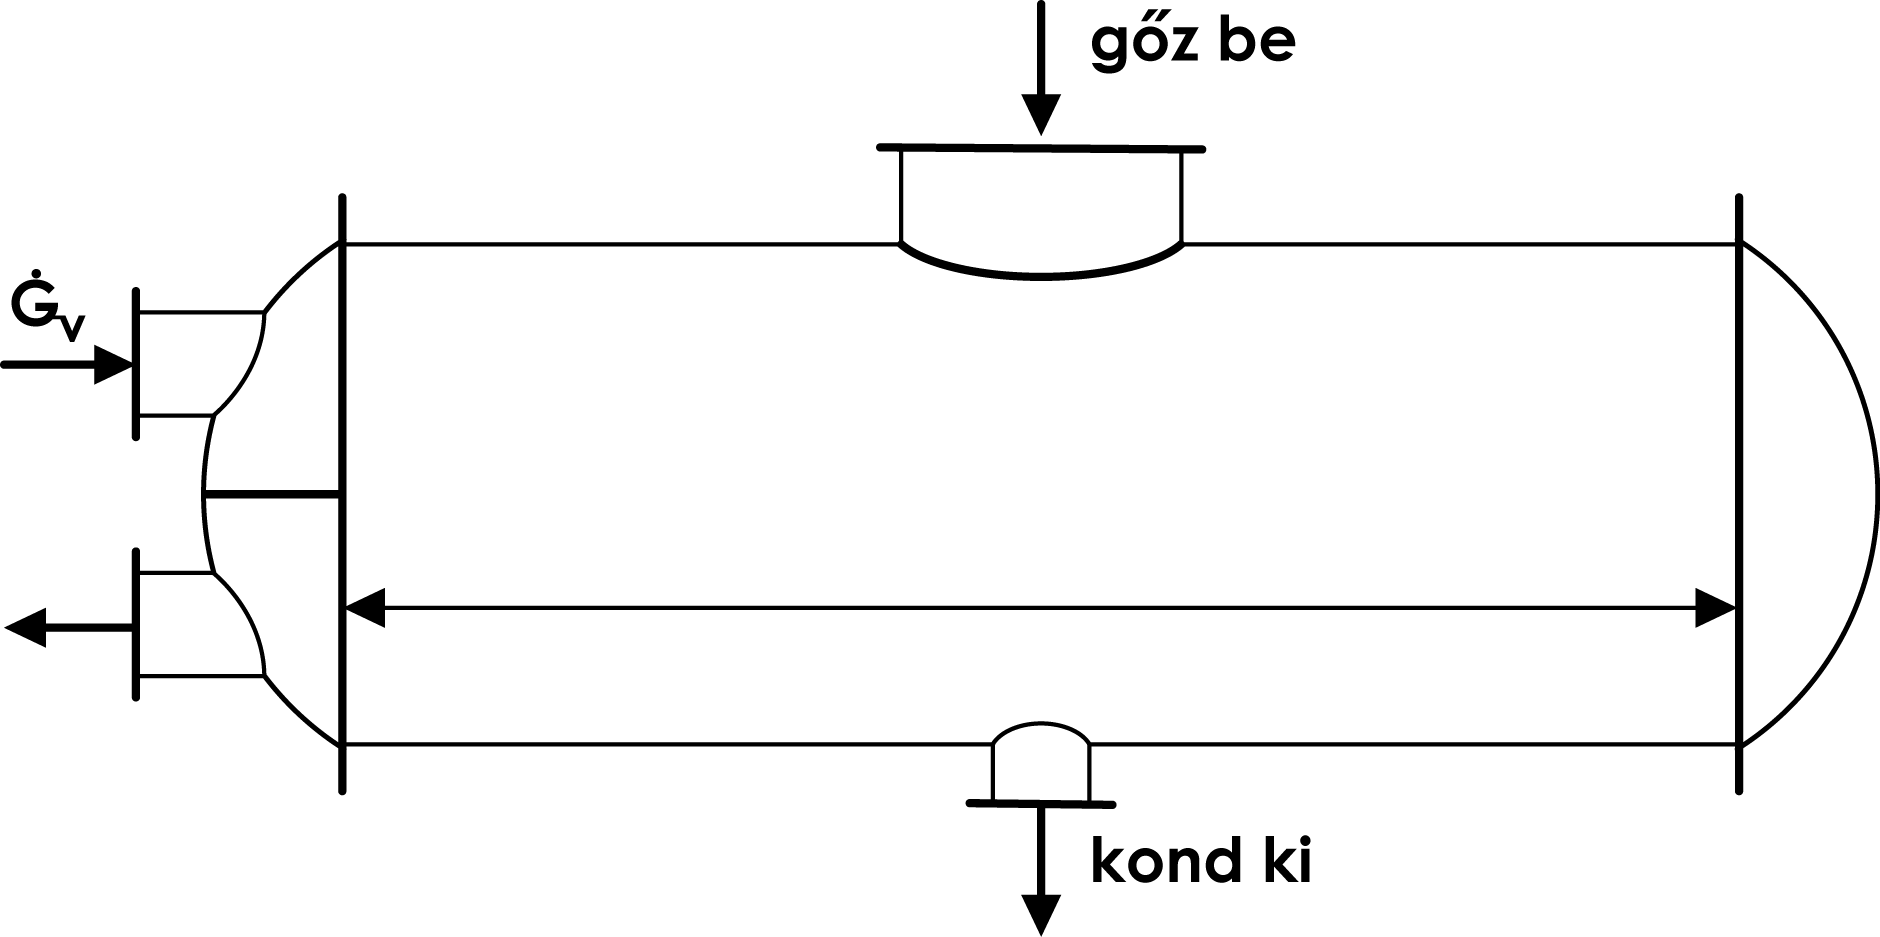
\includegraphics[width=0.5\linewidth]{u9awby123/fig03.png}
	\end{center}
\end{figure}

\begin{figure}[H]
	\begin{center}
		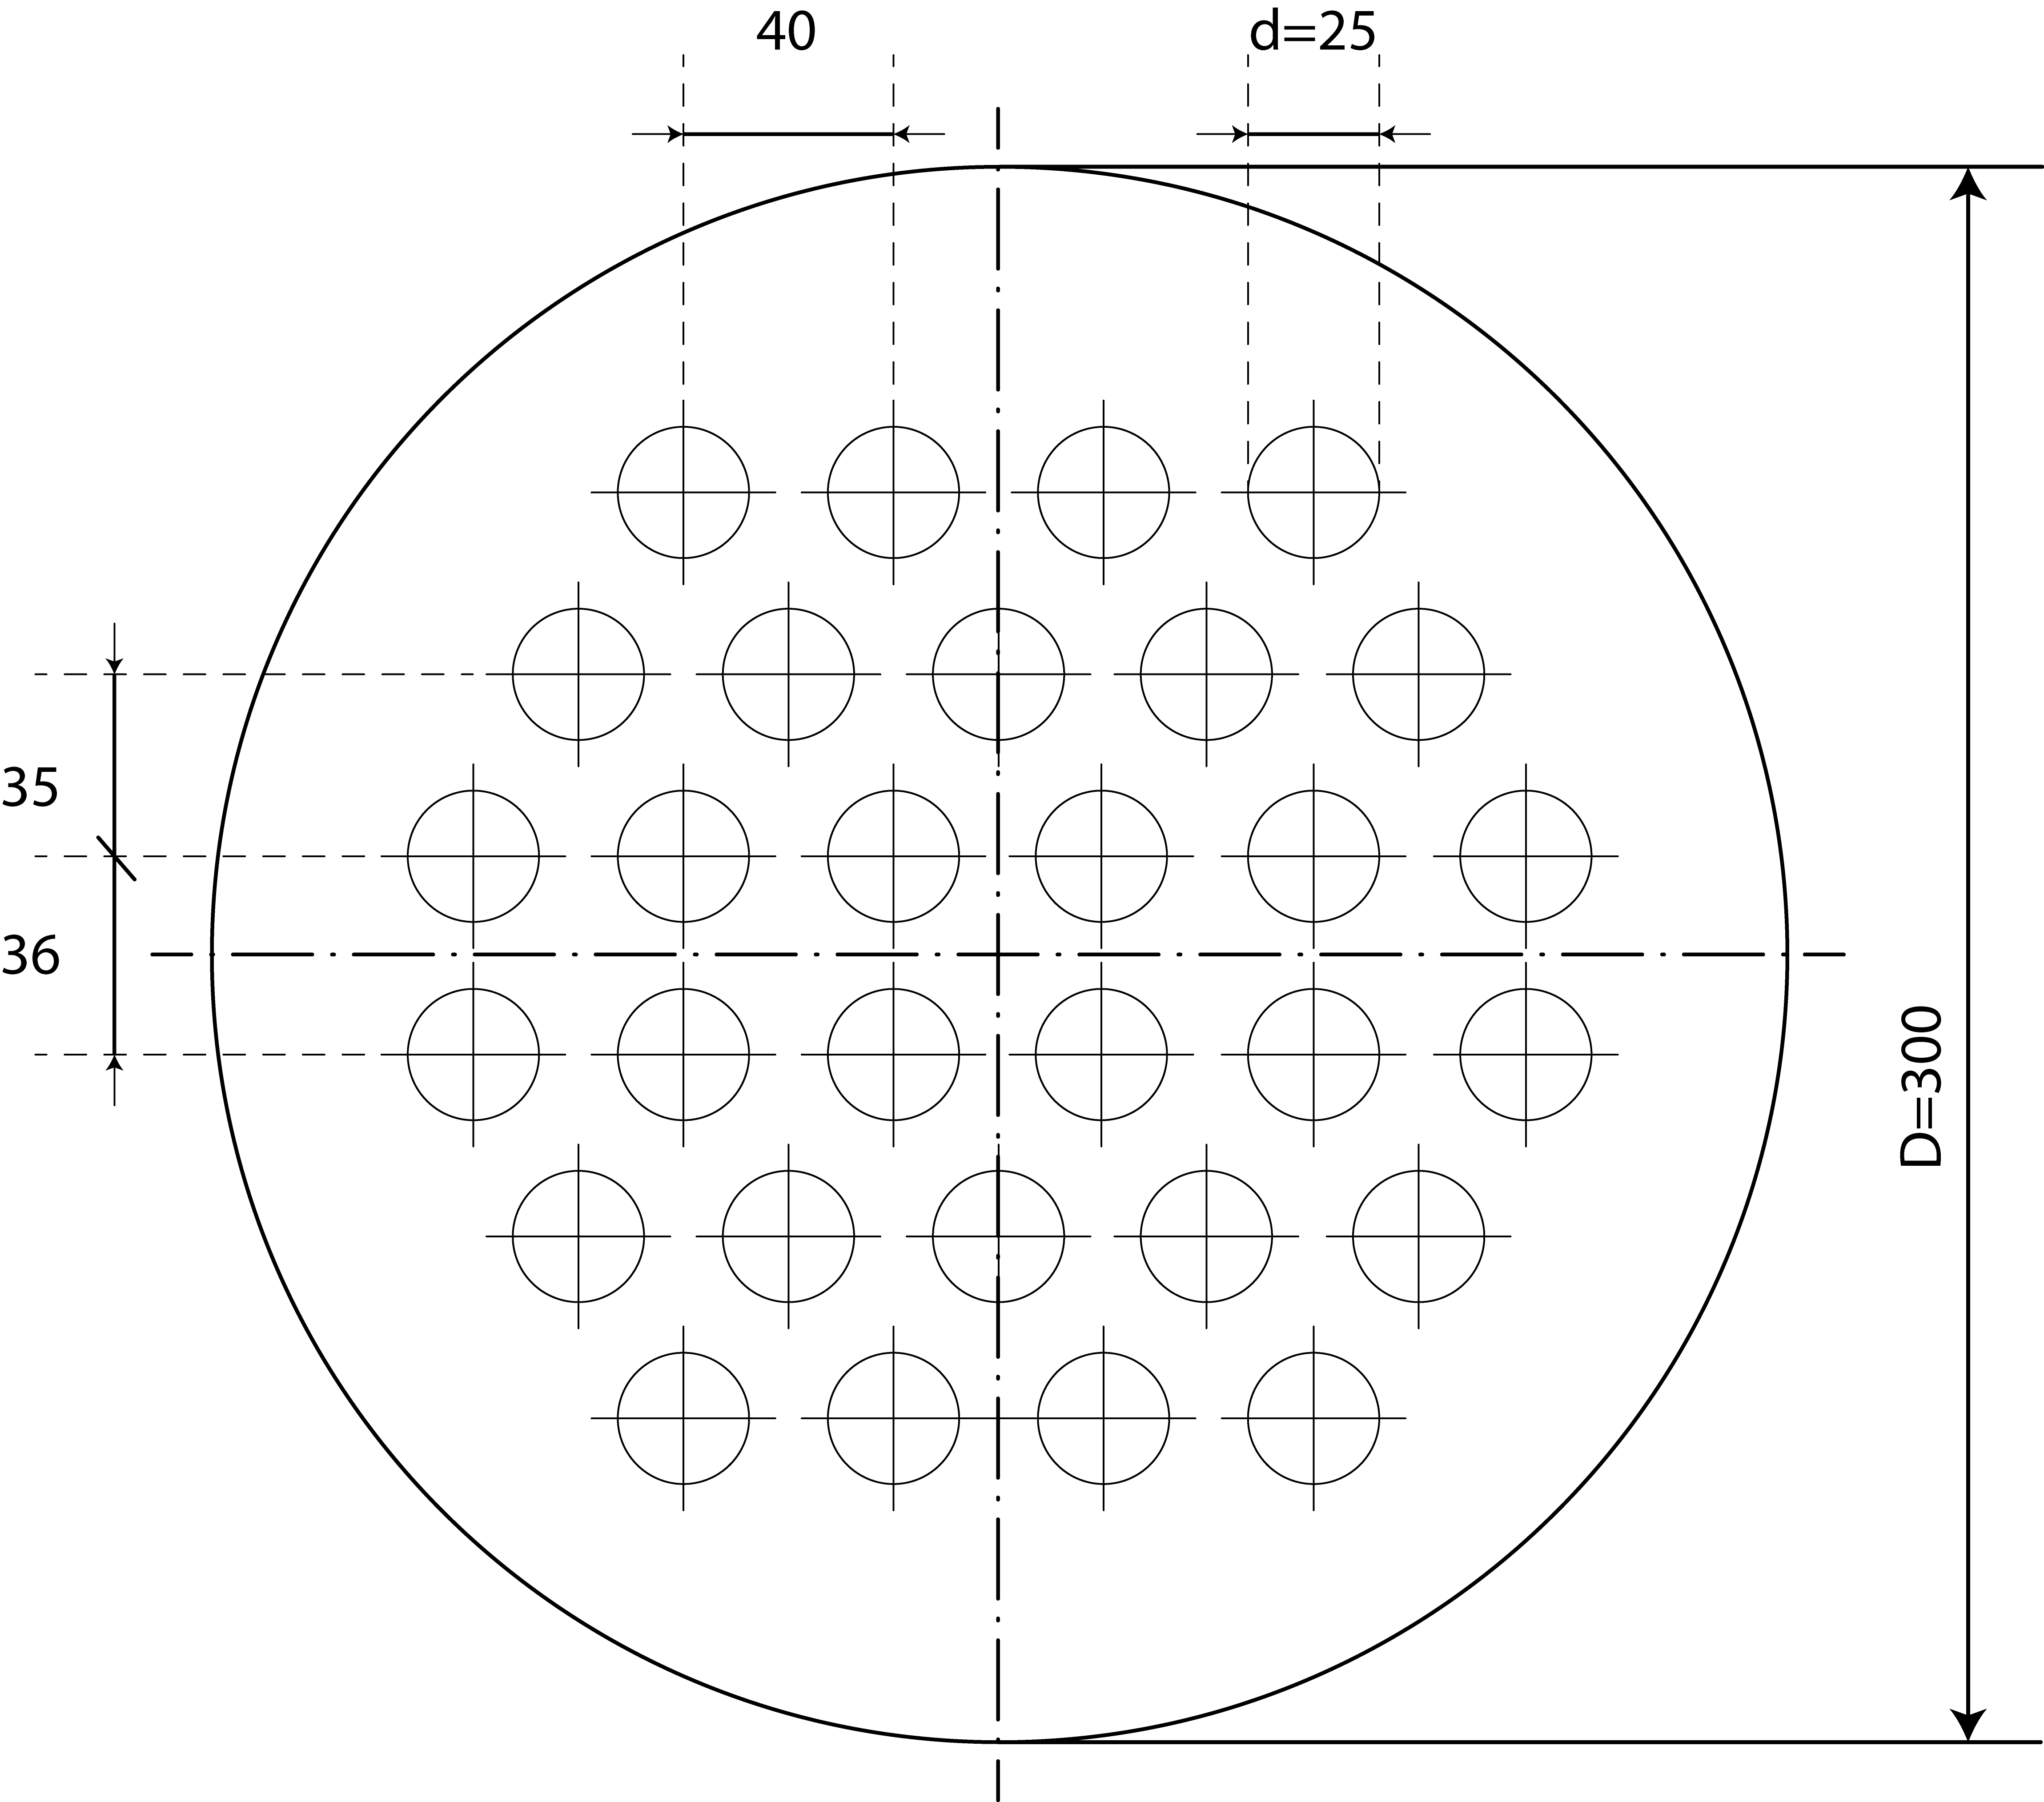
\includegraphics[width=0.5\linewidth]{u9awby123/fig04.png}
	\end{center}
\end{figure}

\vspace{5mm}
$L=\dfrac{43}{30}=1,433$ m

\vspace{5mm}
\noindent
5. A hűtővíz áramlási sebessége (15 db csövön párhuzamosan átáramlik a víz)

\vspace{5mm}
$W_w=\dfrac{V_v}{30\dfrac{d_b^2\pi}{4}3600}=\dfrac{11,0}{30\dfrac{0,02^2 \pi}{4}3600}=$ \underline{0,3242 m/s}

\vspace{5mm}
\noindent
6. Az áramlási jellege a Re szám alapján.

\noindent
a víz közepes hőmérséklete

\vspace{5mm}
$t_m=\dfrac{20+28,56}{2}=$\underline{24,28 °C}

\vspace{5mm}
\noindent
a víz anyagjellemzői ezen hőmérsékleten


 \[
	\left
6		\begin{array}{l}
			\rho_v=997 \textmd{ kg/m}^3\\
			\upsilon_v=0,9025\cdot10^{-6} \textmd{ m}^2/\textmd{s}
		\end{array}
	\right\} \textmd{25 °C-on}
\]


\vspace{5mm}
Re=$\dfrac{wd_b}{\upsilon}=\dfrac{0,3242\cdot0,02}{0,9025\cdot10^{-6}}=7185$; turbulens

\vspace{5mm}
\noindent
7. víz oldalai hőátadási tényező meghatározásához VDI. a Warmeatlas Gb-10 sz.nomogramját használjuk . Pr=6,22 . . . táblázatból

\vspace{5mm}
$\dfrac{d_b}{L}=\dfrac{0,02}{1,433}=1,395*10^{-2}$

\vspace{5mm}
Érvényességi feltételeknek megfelelően

Ezen adatok alapján a nomogramból 

\vspace{5mm}
$\alpha'_v=1744$ W/m$^2$K

\vspace{5mm}
\noindent
8. Ezt az $\dfrac{\nu_{fl}}{n_W}^{0,14}$  - értékkel módosítani kell.

\vspace{5mm}
$\eta_{fl}$=917$\cdot$10$^{-6}$Pa*s; 25 °C-on; $\eta_w$ –kikereséséhez azonban ismerni kel a fal ($t_w$) mérsékletét, ezt eddig nem ismertük. Az $\alpha$ pontos értékét, tehát iterációval határozzuk meg, amihez a fal mérsékletét az alábbi egyenletből számítjuk:

\vspace{5mm}
$\dot{Q}=\alpha_V A (t_w -t_v)$

\vspace{5mm}
$t_w$ = 47,53 °C;  $\eta_w=584,10^{-6}$ Pa$\cdot s$

\vspace{5mm}
$\dfrac{\eta_{fl}}{\eta_{w}}^{0,14}$ = 1,06

\vspace{5mm}
A korrigált $\alpha'_{v}$ tehát

\vspace{5mm}
$\alpha'_{vkorr} = 1,06 \cdot 1744=1848,6$ W/m$^2$K


\begin{figure}[H]
	\begin{center}
		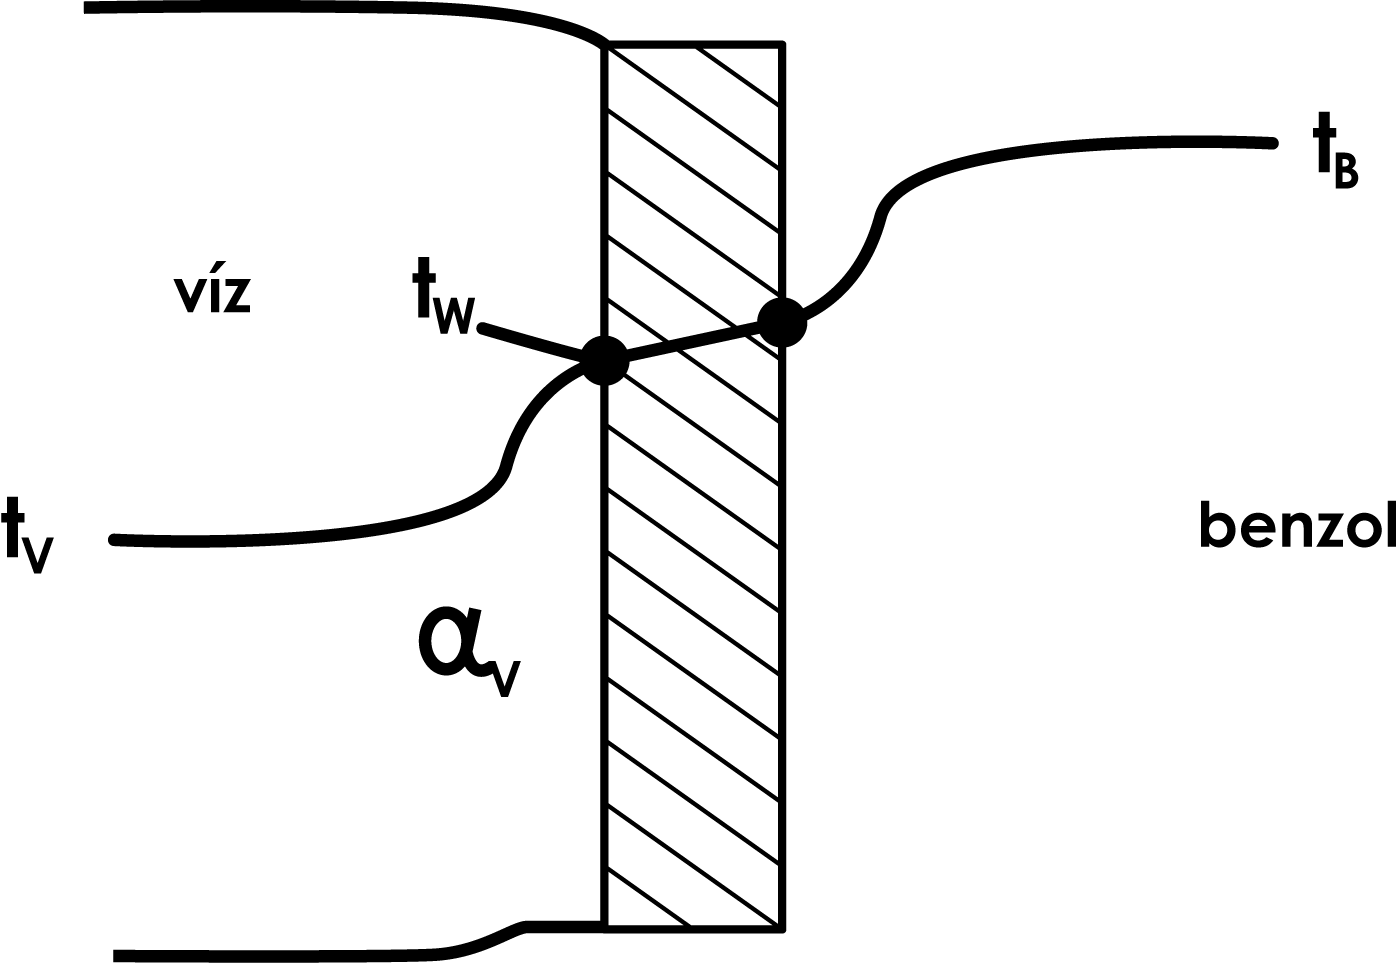
\includegraphics[width=0.5\linewidth]{u9awby123/fig05.png}
	\end{center}
\end{figure}

\vspace{5mm}
\noindent
9. A gőz oldali hőátadási tényező meghatározásához a Ja-5. sz. nomogramot használjuk.

$H=d_k$=0,025 m . . . a csövek külső átmérője

$\Delta t=t_b-t_w=60-47,54=12,56$ °C

$\alpha_{\dot{B}}=2617$ W/m$^2$K

\vspace{5mm}
Ezt az $\alpha$-t vízszintes csövek esetén korrigálni kell 0,77 értékei, tehát 

\vspace{5mm}
$\alpha_{\dot{B}}=0,77 \cdot 2617=2015$ W/m$^2$K

\vspace{5mm}
\noindent
10. Ellenőrizzük azz előzetesen felvett K értékét a most kiszámított alpha-kal;

\vspace{5mm}
$\lambda_{réz}=98,5$ W/mK

\vspace{5mm}
$\kappa"=\dfrac{1}{{\dfrac{1}{\alpha'_{\textmd{vkorr}}}}+\dfrac{\delta}{\lambda}+\dfrac{1}{\alpha_{\dot{B}\textmd{korr}}}}=$\underline{943,6 Wm$^2$K}

\vspace{5mm}
\noindent
11. A 10.-ben számított $\chi$" nem egyezik $\chi$’-val, tehát a számítást meg kell ismételni egy új $\kappa$-val, ez legyen 930.

\vspace{5mm}
$A"=\dfrac{394,2\cdot10^{3}\cdot1000}{930\cdot35,55\cdot3600}=3,31 m^{2}$,

\vspace{5mm}
\noindent
Így 

$l"=\dfrac{3,31}{0,02\cdot\pi}=52,52$ m; $L"=\dfrac{52,52}{30}=$\underline{1,750 m}

\vspace{5mm}
\noindent
Gb-10-ből $\alpha"_v:$

\vspace{5mm}
$\dfrac{d_b}{L"}=0,01143$; $\alpha"_v=$\underline{1756 W/m$^2$K}

\vspace{5mm}
\noindent
A fal hőfokon

\vspace{5mm}
$t"_w=\dfrac{394,2\cdot10^6}{1756\cdot3,31\cdot3600}+24,28=43,2$ °C

\vspace{5mm}
$\eta"_w=626\cdot10^{-6}$ Pa$\cdot$s

\vspace{5mm}
$\dfrac{\eta_{fl}}{\eta"_{w}}^{0,14}=1,055$

\vspace{5mm}
$\alpha"_{vkorr}=1,055\cdot1756=$\underline{1852,6 W/m$^2$K}

\vspace{5mm}
Ja-5-ből $\alpha"_B$:

\vspace{5mm}
$\Delta t"=60-43,2=16,8$ °C; $\alpha"_B=$ 2407 W/m$^2$K

\vspace{5mm}
$\alpha"_{Bkorr}=0,77\cdot2407=1853,7$ W/m$^2$K

\vspace{5mm}
Ezekkel a legújabb $\chi"$' értéke

\vspace{5mm}
\noindent
$\chi"$'=906,5 W/m$^2$K, ami a felvett értékkel elfogadhatóan egyezik. 



